\documentclass[a4paper]{MagicalCV}

% Removing page numbers
\usepackage{fancyhdr}

\usepackage{tikz}
\usetikzlibrary{calc,positioning}
\usepackage[backend=bibtex]{biblatex}
\addbibresource{publications.bib}
 
\pagestyle{fancy}
\fancyhf{}

% Change the geometry
\geometry{left=1.4cm, top=.8cm, right=1.4cm, bottom=1.8cm, footskip=.5cm}

% Defining your colors
\definecolor{VividPurple}{HTML}{3E0097}
\definecolor{SlateGrey}{HTML}{2E2E2E}
\definecolor{LightGrey}{HTML}{666666}
\colorlet{heading}{VividPurple}
\colorlet{accent}{VividPurple}
\colorlet{emphasis}{SlateGrey}
\colorlet{body}{LightGrey}

% Color for highlights
% Awesome Colors: awesome-emerald, awesome-skyblue, awesome-red, awesome-pink, awesome-orange
%                 awesome-nephritis, awesome-concrete, awesome-darknight
\colorlet{awesome}{awesome-purple}

% Set false if you don't want to highlight section with awesome color
\setbool{acvSectionColorHighlight}{true}

% If you would like to change the social information separator from a pipe (|) to something else
\renewcommand{\acvHeaderSocialSep}{\quad\textbar\quad}

% start document
\begin{document}

% Last update time
\lastupdated

% Title name
\namesection{António}{Capela}{
\phone{+351969874351} \email{\href{mailto:acapela96@hotmail.com}{acapela96@hotmail.com}}}

% Cute face
\begin{tikzpicture}[remember picture,overlay]
    \node at ($(current page.north west)+(3cm,-1.6cm)$)[
    circle,
    minimum size=2.5cm,
    path picture={
        \node at (path picture bounding box.center){
            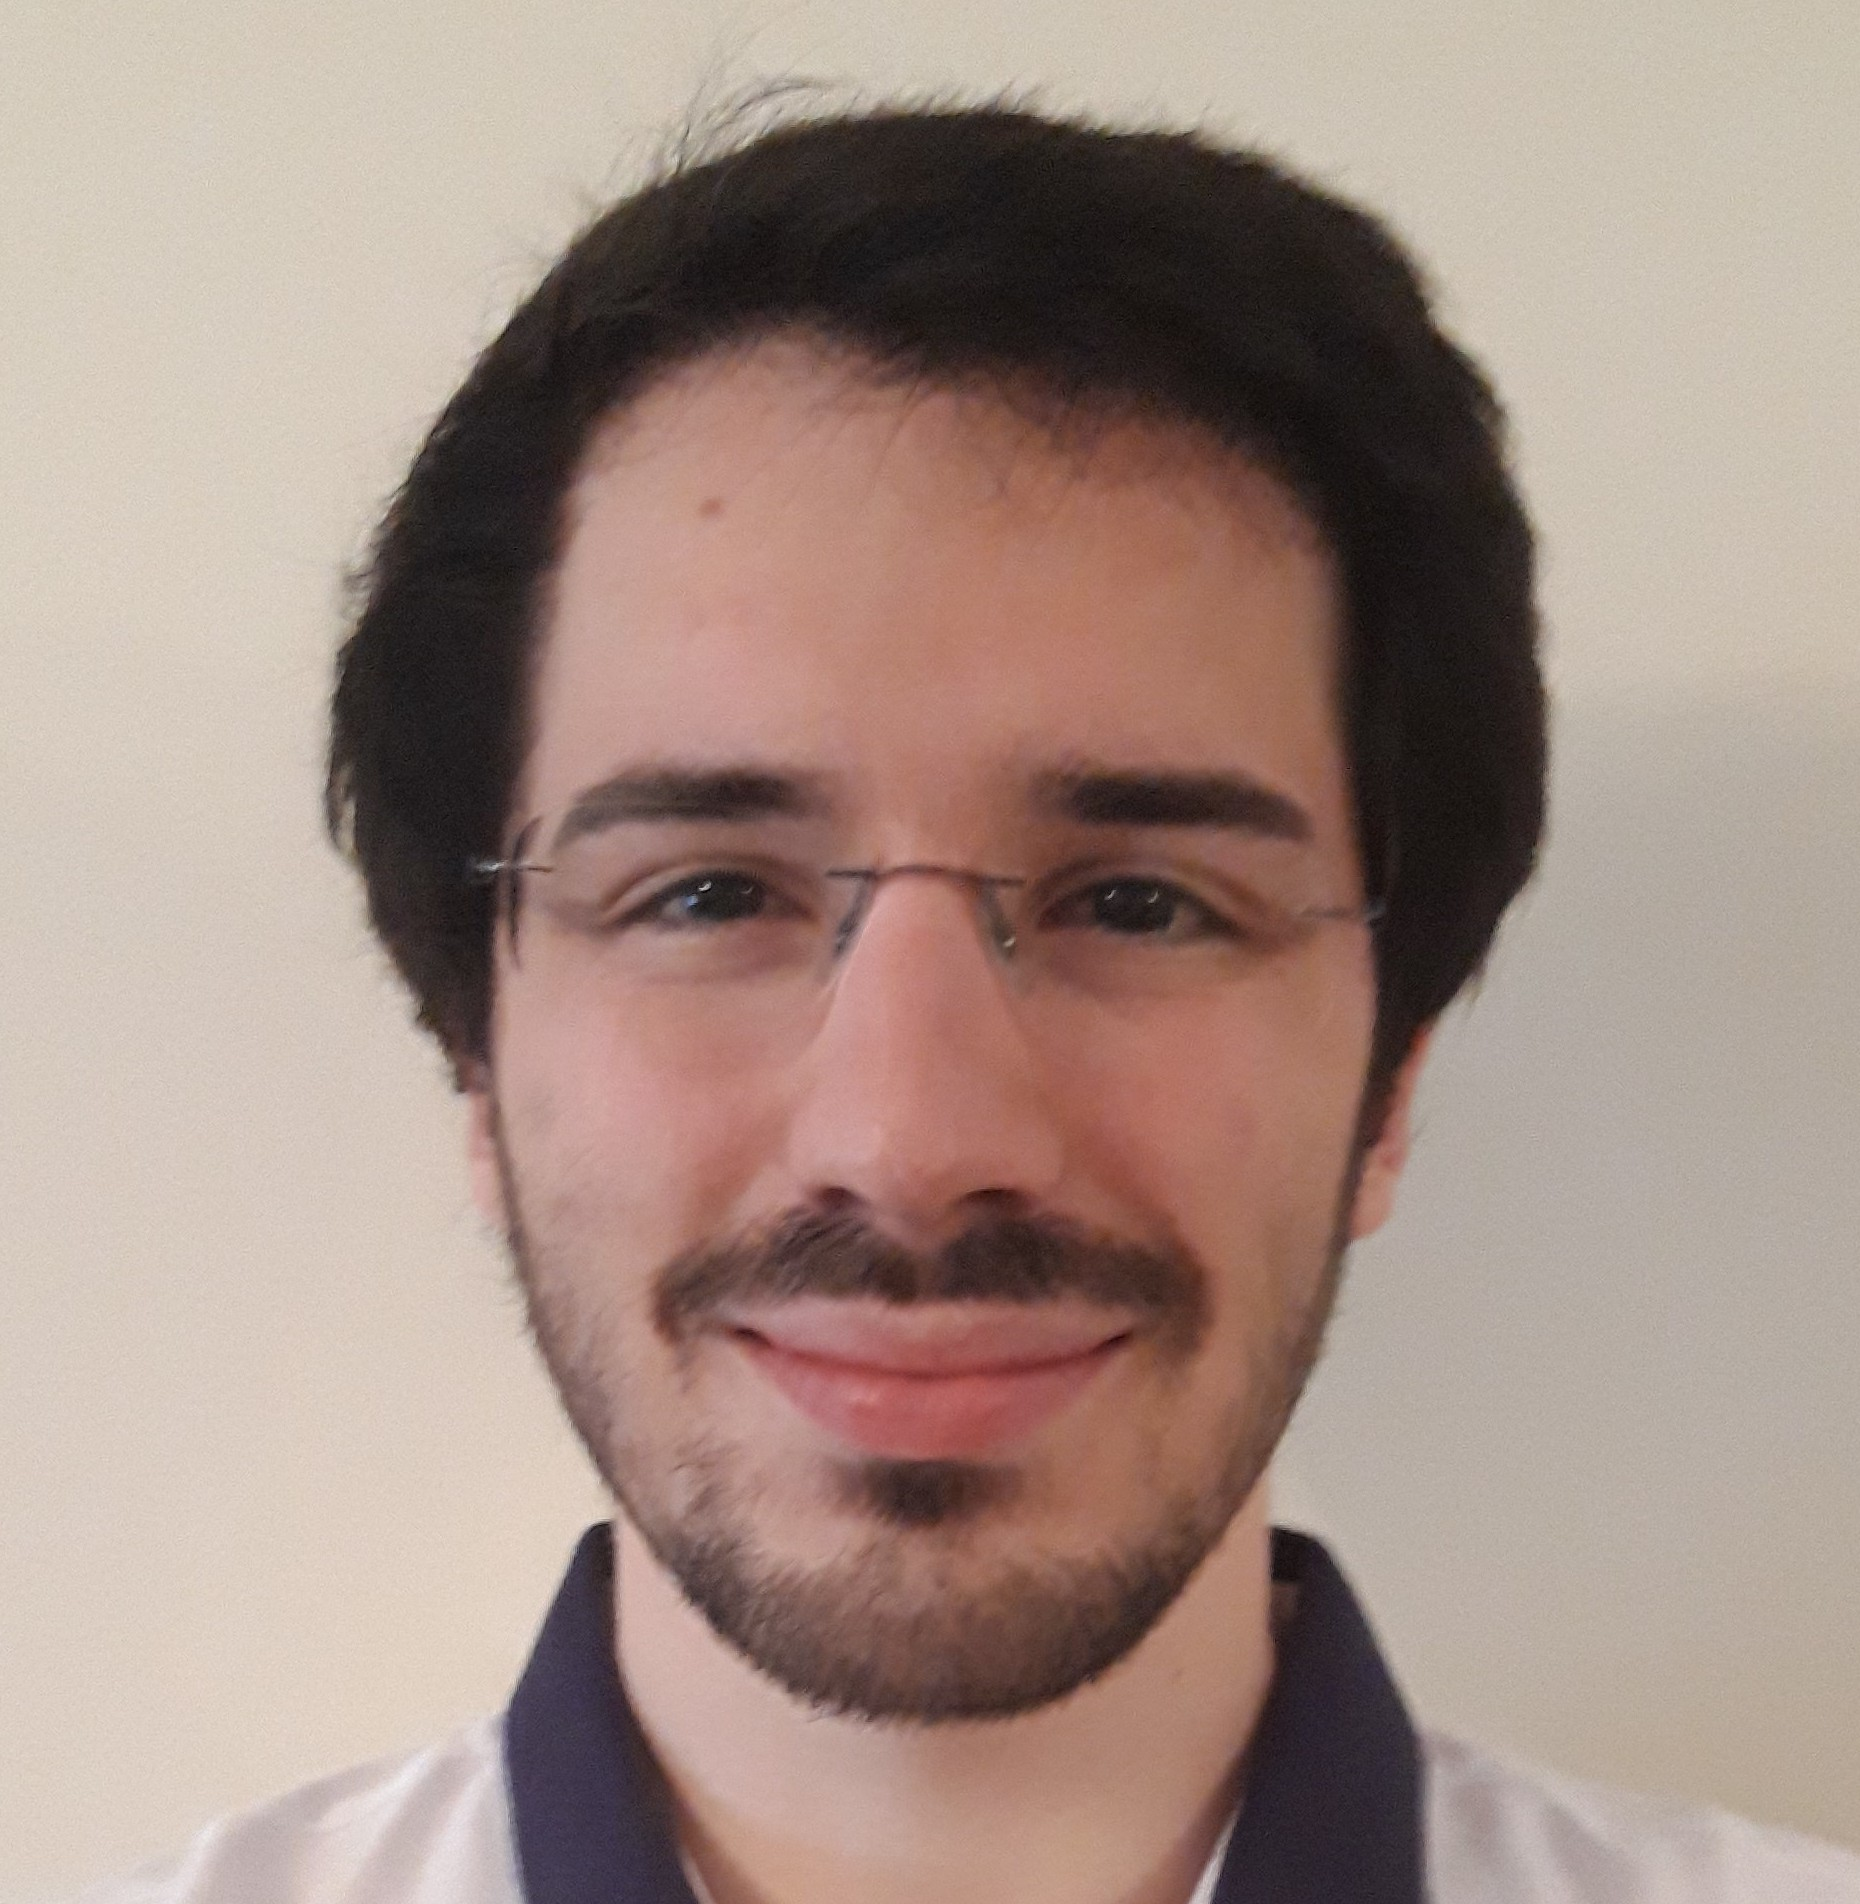
\includegraphics[width=2.5cm]{eu_tipo_passe.jpg}
        };
    }]{};
\end{tikzpicture}

% Column one
\begin{minipage}[t]{0.33\textwidth} 

% Links
\cvsection{Links}

\github{GitHub} \href{https://github.com/antcap96}{\bf antcap96} \\
\linkedin{Linkedin} \href{https://www.linkedin.com/in/appcapela/}{\bf appcapela}
\sectionsep

% Coursework
\cvsection{Coursework}

\subsection{Graduate}
Advanced Algorithms \\
Computability and Complexity \\
Artificial Intelligence \\
Machine Learning \\
Reinforcement Learning \\
Time Series Analysis \\
Probability Theory \\
Statistical Learning \\
\textbf{Dissertation: }
An Adaptive and Transferable Dialog Management System for Social Aware Task Execution \cite{capela2019adaptive}
\sectionsep

% Skills
\cvsection{Skills}

\subsection{Programming}
Python \textbullet{}
Julia \textbullet{}
C \textbullet{}
C++ \textbullet{}
SQL \textbullet{}
Scala
\sectionsep
\subsection{Miscellaneous}
Shell \textbullet{}
LaTeX \textbullet{}
Git \textbullet{}
Microsoft Office \textbullet{}
Confluence

% Languages
\cvsection{Languages} 

\subsection{English}
\descript{C1}
\vspace{\topsep} % Hacky fix for awkward extra vertical space
Certificate obtained by achieving grade A on the FCE exam in 2013.
\sectionsep

\subsection{Portuguese}
\descript{Mother Tongue}
\vspace{\topsep} % Hacky fix for awkward extra vertical space
\sectionsep

% Certificates
\cvsection{Certificates}

\runsubsection{Microsoft -- Azure} \\
\descript{Azure Data Scientist Associate}
\descript{Azure AI Engineer Associate}

% Column two
\end{minipage} 
\hfill
\begin{minipage}[t]{0.66\textwidth} 

% Education
\cvsection{Education} 

\subsection{Instituto Superior Técnico}
\descript{Bachelor's degree in Engineering Physics}
\cvevent{Sep 2017}{Lisbon}
\vspace{\topsep} % Hacky fix for awkward extra vertical space
\sectionsep

\subsection{Instituto Superior Técnico}
\descript{Master's degree in Mathematics and Applications}
\cvevent{Sep 2020}{Lisbon}
\sectionsep

% Experience
\cvsection{Experience}

\runsubsection{Machine Learning Intern} \\
\descript{LIP Summer Internship}
\cvevent{July 2017 -- August 2017}{Lisbon, Portugal} 
\vspace{\topsep} % Hacky fix for awkward extra vertical space
\begin{tightemize}
    \item Data analysis on simulated data of di-Higgs production from CERN's ATLAS experiment.
    \item Development of a Machine Learning model with Neural Networks and Boosted Decision Trees to identify collisions that generate di-Higgs particles.
\end{tightemize}
\sectionsep

\runsubsection{Data Scientist} \\
\descript{Data Scientist Consultant at Xpand-IT}
\cvevent{Oct 2020 -- current}{remote work, Portugal} 
\vspace{\topsep} % Hacky fix for awkward extra vertical space
\begin{tightemize}
    \item Worked with the Data Science team at major portuguese bank for over 1 year. Some of the things I worked on there were: creating ETL pipelines using pyspark that were orchestrated with \href{https://kedro.readthedocs.io/en/stable/index.html}{Kedro} and \href{https://airflow.apache.org}{Apache Airflow}; Development of Machine Learning models to be used by other teams at the bank.
    \item Developed a classification model in Azure Databricks for a major european agency. The model created was a gradient boosting tree (\href{https://lightgbm.readthedocs.io/en/latest/}{LightGBM}) and was implemented as a real time inference model in a Kafka stream.
    \item Worked for an Irish Startup, were we developed an image classification model. The model consisted of a Convolutional Neural Network, implemented with \href{https://keras.io/}{Keras} making use of transfer learning from the VGG16 model.
    \item Performed sentiment analysis using Azure Cognitive Services and keyword extraction with \href{http://yake.inesctec.pt/}{YAKE} to identify causes of complaint in messages.
\end{tightemize}
\sectionsep

% Personal Projects
\cvsection{Personal Projects} 

\runsubsection{\href{https://github.com/antcap96/sqlinpython}{Sqlinpython}} \\
\descript{SQL library in python}
 Inspired by python code containing strings with SQL queries and with the goal of improving my knowledge in: creating a python library, static typing using mypy as well as SQL, I ended up developing a toy library to mimic SQL syntax but using python objects with static checks that ensure the SQL syntax is valid.
\sectionsep

\end{minipage} 

\printbibliography
\end{document}  